\documentclass[12pt,twoside]{article}
\usepackage{weiiszablonzmodyfikowany}
\usepackage{float}
\usepackage{tabularx}
\usepackage{amsmath}
\usepackage{amssymb}
\usepackage{tikz}
\usetikzlibrary{shapes.geometric, arrows.meta, chains, positioning, fit, backgrounds}

% Imię i nazwisko autora projektu
\author{Katarzyna Tylutka}

% Numer indeksu autora (np. 123456)
\studentID{179635}

% Tytuł pracy (należy podać pełny tytul pracy)
\title{Sterowanie robotem balansującym}

% Prowadzący
\supervisor{dr inż. Dawid Kalandyk}

\begin{document}

% strona tytułowa
\maketitle

\blankpage

% spis treści
\tableofcontents

\clearpage
\blankpage

\section{Wstęp}

Celem niniejszej pracy jest opracowanie systemu sterowania dwukołowego robota samobalansującego, zrealizowanego na platformie Raspberry Pi. Robot można traktować jako odwrócony układ wahadłowy: w położeniu górnym jest on niestabilny dynamicznie, dlatego utrzymanie równowagi wymaga ciągłej korekty sygnału sterującego w odpowiedzi na zmiany kąta nachylenia.

W pracy przyjęto następującą metodykę. Najpierw sformułowano model fizyczny i matematyczny układu oraz oszacowano jego parametry na podstawie rzeczywistej konstrukcji. Następnie opisano sposób estymacji stanu robota na podstawie pomiarów z modułu IMU. Na tej podstawie zaprojektowano strategię sterowania opartą na uczeniu ze wzmocnieniem, wytrenowaną w środowisku symulacyjnym, a następnie zaimplementowaną na docelowej platformie sprzętowej.

Przykładem praktycznego zastosowania podobnej idei jest robot Segway --- pojazd samobalansujący wykorzystywany jako środek transportu osobistego. Pokazuje on, że stabilizacja niestabilnego układu mechanicznego jest możliwa przy zastosowaniu odpowiedniego algorytmu sterowania i wiarygodnej informacji o stanie obiektu.

Struktura pracy odpowiada przyjętej metodyce. Rozdział~2 przedstawia model fizyczny robota i jego parametryzację. Rozdział~3 opisuje estymację stanu układu na podstawie danych z czujników. Kolejne rozdziały dotyczą treningu strategii sterowania oraz jej wdrożenia na Raspberry Pi.

\section{Model fizyczny i matematyczny}

W dalszej części pracy układ balansujący zostanie opisany najpierw jako model fizyczny, następnie w postaci równań ruchu, a na końcu poprzez parametry wynikające z rzeczywistej konstrukcji robota. Taki porządek umożliwia przejście od ogólnego opisu zjawiska do modelu możliwego do wykorzystania w sterowaniu.

\subsection{Inverted pendulum}
Model odwróconego wahadła posiada dwa punkty równowagi - jeśli spoczywa w położeniu dolnym jest on stabilny, w przeciwnym wypadku pozostaje on w stanie niestabilności (\cite{str1}). Zadaniem algorytmu jest utrzymanie wahadła w położeniu górnym, tak, aby było ono stabilne. Odbywa się to poprzez odpowiednie sterowanie napięciem silników, o którym decyduje ww. algorytm i agent.

\begin{figure}[ht]%
 \centering%
 \includegraphics[width=6cm]{figures/1.png}%
 \caption{Model odwróconego wahadła i siły na niego działające (źródło: \cite{str2})}%
 \label{Fig:inv_pend}%
\end{figure}

Na rysunku ~\ref{Fig:inv_pend} przedstawiony jest schemat modelu odwróconego wahadła wraz z opisanymi działającymi na niego siłami, gdzie:

\begin{itemize}
    \item M - masa korpusu robota wraz z elektroniką i Raspberry Pi
    \item m - masa kół wraz z silnikami
    \item l - odległość od osi kół do środka ciężkości robota
    \item I - moment bezwładności korpusu względem środka masy
    \item $\theta$ - kąt odchylenia od pionu (mierzony przez filtr komplementarny)
    \item  x - przemieszczenie robota
    \item r - promień kół robota
\end{itemize}

\subsection{Model matematyczny}
\label{sec:model-matematyczny}
Na podstawie źródła \cite{str2} wprowadzić można uproszczone równania ruchu wahadła. Ruch całego układu można opisać za pomocą nieliniowych równań różniczkowych. Po linearyzacji układu wokół punktu równowagi ($\theta = 0$), otrzymujemy przybliżony model matematyczny:
\begin{equation}
(M+m)\ddot{x} + Ml\ddot{\theta}\cos\theta - Ml\dot{\theta}^2\sin\theta = F
\label{wz1}
\end{equation}
\begin{equation}
(I + Ml^2)\ddot{\theta} + Ml\ddot{x}\cos\theta - Mgl\sin\theta = 0
\label{wz2}
\end{equation}

gdzie:

\begin{enumerate}
    \item[-] F - siła napędowa generowana przez koła
    \item[-] $\ddot{\theta}$ - przyspieszenie kątowe (jak szybko zmienia się prędkość przechylania)
    \item[-] $\ddot{x}$ - przyspieszenie liniowe robota 
    \item[-] $\dot{\theta}$ - prędkość kątowa (jak szybko robot się przechyla, odczytywane bezpośrednio z żyroskopu)
    \item[-] równanie opisuje ruch obrotowy korpusu; wpływ napędu jest przenoszony przez sprzężenie z przyspieszeniem liniowym $\ddot{x}$ oraz siłę $F$ w równaniu~\eqref{wz1}
\end{enumerate}

Wzór ~\ref{wz1} jest wzorem liniowym - opisuje co dzieje się z robotem wzdłuż osi x (translacja). 

\begin{enumerate}
    \item[-] $(M+m)\ddot{x}$ i siła potrzebna do nadania przyspieszenia całej masie robota
    \item[-] $Mlcos\theta$ - efekt sprzężenia (gdy góra robota gwałtownie się wychyla ($\theta$), popycha ona dół robota)
    \item[-] $Ml\dot{\theta}^2sin\theta$ - siła odśrodkowa wynikająca z ruchu wahadła
\end{enumerate}

Wzór ~\ref{wz2} opisuje ruch obrotowy (rotację). Można wywnioskować z niego powód, przez który robot się przewraca.

\begin{enumerate}
    \item[-] $(I+Ml^2)\ddot{\theta}$ - moment potrzebny do obrócenia korpusu; $I+Ml^2$ to całkowity moment bezwładności względem osi obrotu
    \item[-] $Ml\ddot{x}cos\theta$ - w przypadku, gdy robot gwałtownie ruszy do przodu ($\ddot{x}$), bezwładność szarpie górą robota w przeciwną stronę
    \item[-] $Mglsin\theta$ - moment grawitacyjny; im większy kąt $\theta$, tym mocniej grawitacja ciągnie robota w dół
\end{enumerate}

W opisywanym układzie sterowanie realizowane jest poprzez siłę napędową $F$ wytwarzaną przez koła robota. Moment obrotowy nie stanowi w tym modelu osobnego, niezależnego wejścia sterującego, lecz jest uwzględniany pośrednio poprzez oddziaływanie siły $F$ na dynamikę translacyjną i sprzężenie z ruchem kątowym korpusu. Dzięki temu równania~\eqref{wz1} i~\eqref{wz2} opisują ten sam układ sterowany siłą działającą wzdłuż osi $x$.


\subsection{Uproszczony model momentu bezwładności robota}

Równania~\eqref{wz1} i~\eqref{wz2} zawierają parametry $M$, $m$, $l$ oraz $I$, które muszą odpowiadać rzeczywistej konstrukcji robota. W niniejszym podrozdziale parametry te oszacowano na podstawie mas poszczególnych elementów oraz ich położenia względem osi obrotu. Warto zaznaczyć, że $l$ opisuje położenie środka ciężkości korpusu nad osią kół, natomiast $I$ --- moment bezwładności elementów obracających się wokół tej osi; są to więc dwie odrębne, lecz powiązane fizycznie wielkości modelu.

W rzeczywistej konstrukcji robota masa nie jest rozłożona równomiernie.
Poszczególne elementy, takie jak silniki, akumulator, Raspberry Pi oraz
obudowa, posiadają różne masy i znajdują się w różnych odległościach od osi
obrotu. Z tego względu całkowity moment bezwładności robota można
rozpatrywać jako sumę momentów bezwładności głównych elementów konstrukcji.

W uproszczonym modelu przyjęto podział robota na cztery główne składowe:

\begin{itemize}
    \item obudowę robota,
    \item dwa silniki wraz z kołami,
    \item akumulator,
    \item Raspberry Pi.
\end{itemize}

W równaniach dynamiki przyjęto podział układu na masę korpusu
\[
M = m_{RPI} + m_{bat} + m_{ob}
\]
oraz masę elementów związanych z osią kół
\[
m = m_{2s}.
\]
Całkowita masa robota jest zatem sumą obu składników.

Masy poszczególnych elementów wynoszą:

\begin{itemize}
    \item masa jednego silnika: $m_s = 0{,}160 \ \text{kg}$,
    \item masa dwóch silników: $m_{2s} = 2 \cdot 0{,}160 = 0{,}320 \ \text{kg}$,
    \item masa Raspberry Pi: $m_{RPI} = 0{,}055 \ \text{kg}$,
    \item masa akumulatora: $m_{bat} = 0{,}250 \ \text{kg}$,
    \item masa obudowy: $m_{ob} = 0{,}466 \ \text{kg}$.
\end{itemize}

Całkowita masa robota wynosi:

\begin{equation}
m_{total} = m_{2s} + m_{RPI} + m_{bat} + m_{ob}
\end{equation}

\begin{equation}
m_{total} = 0{,}320 + 0{,}055 + 0{,}250 + 0{,}466 = 1{,}091 \ \text{kg}
\end{equation}

Całkowity moment bezwładności układu względem osi obrotu (oś kół) zapisano jako sumę momentów bezwładności poszczególnych elementów:

\begin{equation}
I_{total}=I_{ob}+I_{bat}+I_{RPI}+I_{2s}
\label{eq:I_total}
\end{equation}

gdzie:

\begin{itemize}
    \item $I_{ob}$ --- moment bezwładności obudowy,
    \item $I_{bat}$ --- moment bezwładności akumulatora,
    \item $I_{RPI}$ --- moment bezwładności Raspberry Pi,
    \item $I_{2s}$ --- moment bezwładności dwóch silników wraz z kołami.
\end{itemize}

Wysokości elementów nad podłożem (oś obrotu w przybliżeniu na poziomie podłogi) przyjęto na podstawie rzutu konstrukcyjnego:

\begin{itemize}
    \item dolna krawędź obudowy nad podłożem: $8{,}3\ \mathrm{mm}$,
    \item wymiary obudowy: długość $L = 155\ \mathrm{mm}$, szerokość $W = 100{,}35\ \mathrm{mm}$, wysokość $h = 160\ \mathrm{mm}$,
    \item akumulator: $108\ \mathrm{mm}$ nad dolną krawędzią obudowy,
    \item Raspberry Pi: $135\ \mathrm{mm}$ nad dolną krawędzią obudowy,
    \item silniki: przy dolnej podstawie obudowy; środek masy układu silnik--koło przyjęto na wysokości osi kół ($r = 33\ \mathrm{mm}$).
\end{itemize}

Odpowiadające odległości osi obrotu od środków mas wynoszą:
$r_{ob} = 88{,}3\ \mathrm{mm}$, $r_{bat} = 116{,}3\ \mathrm{mm}$, $r_{RPI} = 143{,}3\ \mathrm{mm}$, $r_{2s} = 33\ \mathrm{mm}$.

Obudowę robota przybliżono jako prostopadłościan obracający się względem osi
przechodzącej przez środek masy. Jej moment bezwładności można więc obliczyć
ze wzoru:

\begin{equation}
I_{o}=\frac{1}{12}m_{ob}(h^2+L^2)
\end{equation}

gdzie $h$ oznacza wysokość obudowy, natomiast $L$ jej długość w płaszczyźnie
ruchu wychylenia (oś obrotu jest równoległa do szerokości $W$).


Lecz trzeba wziąć pod uwagę fakt, że oś obrotowa nie będzie przechodziła idealnie przez środek bryły, dlatego trzeba użyć twierdzenia Steinera

\begin{equation}
I_{ob}=I_{o} + m_{ob}r^2_{ob}
\end{equation}

gdzie $I_{o}$ to moment bezwładności względem środka masy obudowy, a $r_{ob}$ to odległość środka ciężkości obudowy od osi obrotu.

Pozostałe elementy potraktowano jako masy skupione. Dla takiego uproszczenia
moment bezwładności pojedynczego elementu opisuje zależność:

\begin{equation}
I_i=m_i r_i^2
\end{equation}

gdzie $m_i$ oznacza masę danego elementu, natomiast $r_i$ jego odległość od osi
obrotu.

Moment bezwładności obudowy wynosi:

\begin{equation}
I_{o}=\frac{1}{12} \cdot 0{,}466 \cdot (0{,}16^2 + 0{,}155^2) = 0{,}001927\ \mathrm{kg{\cdot}m^2}
\end{equation}

\begin{equation}
I_{ob}=I_{o} + m_{ob}\,r_{ob}^2 = 0{,}001927 + 0{,}466 \cdot 0{,}0883^2 = 0{,}00556\ \mathrm{kg{\cdot}m^2}
\end{equation}

Moment bezwładności akumulatora wynosi:

\begin{equation}
I_{bat}=m_{bat}r_{bat}^2
\end{equation}

\begin{equation}
I_{bat}=0{,}250 \cdot 0{,}1163^2 = 0{,}00338\ \mathrm{kg{\cdot}m^2}
\end{equation}

Moment bezwładności Raspberry Pi wynosi:

\begin{equation}
I_{RPI}=m_{RPI}r_{RPI}^2
\end{equation}

\begin{equation}
I_{RPI}=0{,}055 \cdot 0{,}1433^2 = 0{,}00113\ \mathrm{kg{\cdot}m^2}
\end{equation}

Moment bezwładności dwóch silników (jako masy skupionej na wysokości osi kół) wynosi:

\begin{equation}
I_{2s}=m_{2s}\,r_{2s}^2 = 0{,}320 \cdot 0{,}033^2 = 0{,}00035\ \mathrm{kg{\cdot}m^2}
\end{equation}

Po podstawieniu wszystkich składowych całkowity moment bezwładności robota
można zapisać w postaci:

\begin{equation}
I_{total}=0{,}00556+0{,}00338+0{,}00113+0{,}00035 \approx 0{,}0104\ \mathrm{kg{\cdot}m^2}
\end{equation}

Wkład silników jest niewielki, ponieważ ich środek masy leży blisko osi obrotu.
Gdyby przyjąć silniki wyłącznie na wysokości podstawy obudowy ($r_{2s}=8{,}3\ \mathrm{mm}$),
otrzymano by $I_{2s} \approx 2{,}2 \cdot 10^{-5}\ \mathrm{kg{\cdot}m^2}$, czyli wartość pomijalną.
Warto zaznaczyć, że $I_{total}$ wyznaczono względem osi kół; w równaniu~\eqref{wz2}
odpowiada to momentowi bezwładności całego układu względem osi wahadła.


Tak zdefiniowany model pozwala uwzględnić nie tylko całkowitą masę robota, ale
również rozmieszczenie jego najważniejszych elementów względem osi obrotu.
Jest to istotne, ponieważ element o większej masie położony dalej od osi
obrotu silniej zwiększa moment bezwładności niż element o tej samej masie
znajdujący się bliżej osi.

Na podstawie przyjętego podziału konstrukcji na elementy składowe wyznaczono zarówno całkowitą masę robota, jak i jego moment bezwładności względem osi obrotu. Otrzymane wartości stanowią parametry wejściowe modelu matematycznego z podrozdziału~\ref{sec:model-matematyczny}. Szczegółowy opis rozmieszczenia tych elementów w obudowie --- uzasadniający przyjęte odległości $r_{ob}$, $r_{bat}$ i $r_{RPI}$ --- przedstawiono w podrozdziale następnym.

\subsection{Fizyczna budowa robota}

Konstrukcja mechaniczna robota została zaprojektowana tak, aby jego rozkład mas był zgodny z założeniami modelu opisanego w podrozdziale poprzednim. Umiejscowienie poszczególnych elementów nie jest więc wyłącznie kwestią montażową, lecz bezpośrednio wpływa na parametry $l$ i $I$ wykorzystywane w równaniach ruchu.

Korpus robota charakteryzuje się formą prostopadłościanu ze zwężeniem w dolnej partii konstrukcji, co przedstawiono na rys. \ref{Fig:obudowa1}.

\begin{figure}[ht]%
 \centering%
 \includegraphics[width=9cm]{figures/2.jpg}%
 \caption{Projekt obudowy robota}%
 \label{Fig:obudowa1}%
\end{figure}

W środku konstrukcji znajdują się miejsca na wsuwane półki (\ref{Fig:obudowa2}):
\begin{itemize}
    \item Poziom dolny --- dolna platforma przeznaczona jest na akumulator zasilający. Umieszczenie akumulatora w najniższej części konstrukcji jest zabiegiem celowym: obniża ono środek ciężkości korpusu i zmniejsza moment bezwładności względem osi kół, co sprzyja stabilizacji pionowej.
    \item Poziom górny: Górna platforma dedykowana jest jednostce
obliczeniowej, mikrokomputerowi Raspberry Pi. Fizyczna separacja
warstwy logicznej od zasilającej minimalizuje ryzyko zakłóceń
elektromagnetycznych oraz zapewnia lepsze chłodzenie procesora
sterującego.
\end{itemize}

\begin{figure}[ht]%
 \centering%
 \includegraphics[width=9cm]{figures/3.jpg}%
 \caption{Rzut przedni obudowy, gdzie widoczne są miejsca na wsuwane półki}%
 \label{Fig:obudowa2}%
\end{figure}

W górnej części obudowy znajduje się dedykowane miejsce na dwa moduły żyroskopowe (IMU - moduł, który integruje 3-osiowy akcelerometr i 3-osiowy żyroskop) PCS10-BMI160 (\ref{Fig:obudowa3}). Zamontowanie ich właśnie w takim położeniu pozwala na lepsze odczytanie przechylenia względem pionu.

\begin{figure}[ht]%
 \centering%
 \includegraphics[width=15cm]{figures/4.jpg}%
 \caption{Dedykowane miejsce na moduł IMU}%
 \label{Fig:obudowa3}%
\end{figure}

Zastosowane rozmieszczenie czujników jest zgodne z przyjętą metodyką modelowania: pomiar wychylenia wykonywany jest w górnej części konstrukcji, czyli w rejonie, w którym występuje dominujący ruch kątowy korpusu. Dzięki temu dane z IMU mogą być wykorzystane do estymacji stanu układu opisanej w rozdziale~3.

W niniejszym rozdziale przedstawiono pełną ścieżkę modelowania robota balansującego: od schematu fizycznego i równań ruchu, przez oszacowanie parametrów masowych i bezwładnościowych, po opis konstrukcji uzasadniający przyjęte założenia. Uzyskany model stanowi podstawę dalszych rozważań dotyczących estymacji stanu oraz syntezy algorytmu sterowania.

\newpage



\section{Teoria}

Model matematyczny przedstawiony w rozdziale poprzednim wymaga bieżącej znajomości stanu układu, a w szczególności kąta nachylenia $\theta$ oraz prędkości kątowej $\dot{\theta}$. W praktyce wielkości te nie są mierzone bezpośrednio, lecz wyznaczane na podstawie sygnałów pochodzących z modułu IMU. W niniejszym rozdziale opisano związane z tym problemy pomiarowe oraz metodę ich rozwiązania wykorzystaną w implementacji programowej.

\subsection{Wyzwania w zakresie estymacji stanu: szum i dryf czujników}
Robot samobalansujący opiera swoją wiedzę o świecie na module IMU. Dane te są jednak obarczone błędami wynikającymi z natury czujników:
\begin{itemize}
    \item Akcelerometr - pozwala wyznaczyć kąt nachylenia na podstawie wektora grawitacji. Jest bardzo stabilny na przestrzeni dłuższego czasu, ale niezwykle podatny na szum wywołany np. wibracjami silników i gwałtownymi ruchami robota.
    \item Żyroskop --- mierzy prędkość kątową $\dot{\theta}$. Przez całkowanie tej wartości można uzyskać kąt nachylenia. Czujnik ten jest bardziej użyteczny przy szybkich ruchach, jednak podlega zjawisku dryfu: z czasem błąd całkowania narasta i mimo że robot pozostaje w pionie, estymowany kąt może odbiegać od rzeczywistego.
\end{itemize}

Żaden z czujników osobno nie zapewnia wiarygodnej estymacji stanu przez cały czas pracy układu. Z tego względu konieczne jest połączenie obu źródeł informacji w jeden sygnał sterowniczy, co realizuje filtr komplementarny opisany w podrozdziale następnym.

\subsection{Filtr komplementarny - fuzja danych}
W celu uzyskania wiarygodnego kąta $\theta$, wykorzystany został filtr komplementarny - algorytm fuzji danych, który łączy zalety obu czujników, działając jak filtr dolnoprzepustowy dla akcelerometru i górnoprzepustowy dla żyroskopu. Matematycznie filtr ten można przedstawić za pomocą wzoru \ref{wz4}. Dzięki przepuszczeniu danych z modułu IMU, $\theta_n$ jest sygnałem czystym, szybkim i pozbawionym dryfu.
\begin{equation}
\theta_{n} = \alpha \cdot (\theta_{n-1} + \dot{\theta}_{gyro} \cdot dt) + (1 - \alpha) \cdot \theta_{acc}
\label{wz4}
\end{equation}

Filtr komplementarny łączy zalety obu czujników: akcelerometru, którego wpływ dominuje przy niskich częstotliwościach, oraz żyroskopu, odpowiedzialnego za szybką reakcję na zmiany położenia. W efekcie otrzymuje się estymowany kąt $\theta_n$, który może zostać wykorzystany w dalszej części algorytmu sterowania.

\subsection{Implementacja pętli sterowania}

Estymowany kąt $\theta_n$ oraz prędkość kątowa $\dot{\theta}$ uzyskana z żyroskopu stanowią podstawowe informacje o stanie robota wykorzystywane w pętli sterowania. Na ich podstawie algorytm sterujący generuje sygnał napędowy, który --- poprzez sterownik silników --- wpływa na dynamikę układu opisaną w rozdziale~2.

Implementacja programowa realizuje tę zależność w postaci cyklicznie wykonywanej pętli sterowania. Dzięki żyroskopowi BMI160 surowa prędkość kątowa jest dostępna natychmiast po odczytaniu rejestrów żyroskopu i przemnożeniu ich przez odpowiednią skalę. Ogólny przebieg programu można podzielić na trzy fazy:
\begin{enumerate}
    \item \textbf{Inicjalizacja} - uruchomienie pinów GPIO, kalibracja sensorów BMI160
    \item \textbf{Główna pętla} - cykliczne odczytywanie danych, przekazywanie ich do filtra, a następnie przetransformowanie na sygnał i wysłanie do silników.
    \item \textbf{Zatrzymanie} --- określenie końca pracy programu po wykryciu upadku robota.
\end{enumerate}

Przepływ informacji w programie sterującym przedstawiono schematycznie na rys.~\ref{Fig:sch_blok}. Sygnał z czujnika BMI160 jest najpierw poddawany filtracji komplementarnej, a następnie wykorzystywany do wyznaczenia sygnału sterującego silnikami.

\begin{figure}[ht]%
 \centering%
 \includegraphics[width=8cm]{figures/5.png}%
 \caption{Schemat blokowy programu}%
 \label{Fig:sch_blok}%
\end{figure}

Podczas procesu inicjalizacji konieczne jest zapewnienie nieruchomego położenia robota, ponieważ kalibracja żyroskopu BMI160 polega na wyznaczeniu przesunięcia dla prędkości kątowej. Nawet niewielkie drgania lub ruch konstrukcji mogą powodować błędne wyznaczenie punktu odniesienia, co skutkuje narastającym błędem estymacji kąta podczas pracy algorytmu. Jednym z rozważanych rozwiązań jest zastosowanie dedykowanego stojaka stabilizującego robota w pozycji pionowej na czas uruchamiania i kalibracji układu pomiarowego.

Implementacja kodu opiera się na pętli sterowania, gdzie kluczowym elementem jest synchronizacja czasowa ($dt$), która zapewnia stabilność całkowania danych z żyroskopu. Schemat blokowy na rys.~\ref{Fig:sch_blok} ilustruje przepływ informacji od surowego sygnału z sensora BMI160, przez filtrację komplementarną, aż po wygenerowanie sygnału PWM sterującego momentem obrotowym silników.

Przedstawiona struktura programu zapewnia powiązanie warstwy pomiarowej z warstwą sterowania. Estymacja stanu na podstawie danych z IMU umożliwia bieżącą ocenę położenia robota, a cykliczna pętla sterowania pozwala na szybką reakcję na zmiany kąta nachylenia. Rozwiązanie to stanowi podstawę implementacyjną dla algorytmu uczenia ze wzmocnieniem omówionego w dalszej części pracy, w którym decyzje sterujące są wyznaczane na podstawie obserwacji stanu układu, a nie klasycznego regulatora PID.


\section{Uczenie ze wzmocnieniem w środowisku symulacyjnym}

W ramach projektu zaimplementowano autorskie środowisko symulacyjne w języku Python, które odwzorowuje dynamikę odwróconego wahadła opisaną wcześniej przedstawionymi równaniami różniczkowymi. Takie podejście zdecydowanie ułatwiło fazę testowania i uczenia algorytmu. Dodatkowo pozwoliło na przeprowadzenie tysięcy epizodów uczenia w krótkim czasie, bez ryzyka fizycznego uszkodzenia prototypu.

\subsection{Definicja procesu decyzyjnego (MDP)}
Aby algorytm RL mógł skutecznie sterować robotem, zdefiniowano kluczowe komponenty procesu:
\begin{itemize}
    \item \textbf{Stan} - wektor obserwacji przekazywany do agenta, obejmujący kąt nachylenia $\theta$ oraz prędkość kątową $\dot{\theta}$.
    \item \textbf{Akcja} - decyzja podejmowana przez agenta, przekładająca się na wartość sygnału sterującego silnikami (np. współczynnik wypełnienia PWM).
    \item \textbf{Funkcja Nagrody} - mechanizm motywujący agenta. W projekcie zastosowano funkcję premiującą minimalizację błędu kątowego (utrzymywanie pionu) oraz nakładającą wysoką karę w przypadku upadku robota ($|\theta| > 35^{\circ}$).
    
\end{itemize}
W praktyce ograniczenie kąta do wartości 35$^{\circ}$ zwiększa bezpieczeństwo działania robota oraz pozwala uniknąć stanów, z których odzyskanie równowagi byłoby niemożliwe ze względu na ograniczenia momentu obrotowego silników.

\subsection{Regulator PID jako fundament}
Klasyczny regulator PID został wykorzystany jako punkt odniesienia dla algorytmów RL. Pozwoliło to na analizę porównawczą "inteligencji" wypracowanej przez agenta względem deterministycznego algorytmu sterowania. Parametry $K_p, K_i, K_d$ zdefiniowano następująco:

\begin{enumerate}
    \item[-] $K_p$ (Wzmocnienie proporcjonalne) – odpowiada za natychmiastową reakcję na błąd. W RL odpowiada to bezpośredniej zależności między stanem a siłą akcji.
    \item[-] $K_i$ (Wzmocnienie całkujące) – niweluje błąd statyczny wynikający z asymetrii konstrukcji. Agent RL uczy się tej kompensacji poprzez długofalową optymalizację sumy nagród.
    \item[-] $K_d$ (Wzmocnienie różniczkujące) – działa jak tłumik, przewidując kierunek upadku na podstawie prędkości kątowej z żyroskopu.
\end{enumerate}

Regulator PID może pełnić również dodatkową rolę źródła danych treningowych dla sieci neuronowej. W przypadku stabilnej pracy regulatora na rzeczywistym robocie możliwe jest rejestrowanie par stan-akcja, gdzie stan opisuje aktualne położenie robota, a akcją jest sygnał sterujący wygenerowany przez regulator PID. Tak przygotowany zbiór danych może zostać wykorzystany do wstępnego uczenia sieci neuronowej metodą imitacji zachowania regulatora klasycznego, co pozwala skrócić czas późniejszego uczenia ze wzmocnieniem oraz poprawić stabilność początkowej polityki sterowania.

\subsection{Środowisko symulacji}
Przed rozpoczęciem procesu uczenia konieczne było określenie parametrów fizycznych modelu oraz konfiguracji bazowego algorytmu sterowania PID, stanowiącego punkt odniesienia dla metod uczenia ze wzmocnieniem. Dopiero po zdefiniowaniu tych parametrów możliwe było utworzenie środowiska symulacyjnego odwzorowującego dynamikę rzeczywistego robota.

Przed implementacją algorytmów RL (SAC i PPO), konieczne było stworzenie wirtualnego świata dla robota w celu wykonywania testów, dobierania parametrów i uczenia sieci neuronowej. Środowisko to jest deterministyczne - te same siły zawsze dają ten sam efekt. Prawdziwy robot jest natomiast stochastyczny z powodu występowania szumów i tarcia zatem symulacja jest bardzo dobrym polem doświadczalnym.
\newline
Klasa InvertedPendulumEnv (environment) składa się łącznie z 3 funkcji:
\begin{enumerate}
    \item \textbf{\_\_init\_\_(self)} - listing \ref{listP1} - ustalane są parametry fizyczne (w tym przyspieszenie ziemskie, przybliżona masa kół i silników, moment bezwładności, krok czasowy symulacji, itp.)

\begin{lstlisting}[language=Python, caption=Inicjalizacja parametrów, label=listP1]
class InvertedPendulumEnv:
    def __init__(self):
        self.g = 9.81      # przyspieszenie ziemskie
        self.m = 0.2       # masa kol wraz z silnikami [
        self.M = 0.8       # masa korpusu (elektronika + Raspberry Pi) 
        self.l = 0.15      # odleglosc do srodka ciezkosci 
        self.I = 0.002     # moment bezwladnosci korpusu 
        self.r = 0.033     # promien kol robota 
        self.dt = 0.01     # krok czasowy (10ms)
        
        self.theta_max = np.radians(35) # granica upadku (theta_max)
        self.state = None # stan [x, x_dot, theta, theta_dot]

        self.reset()
\end{lstlisting}

    \item \textbf{reset(self)} - listing \ref{listP2} - funkcja przywracająca stan poczatkowy z lekkim wychyleniem

\begin{lstlisting}[language=Python, caption=Funkcja reset, label=listP2]
def reset(self):
    # theta inicjalizowane jako mały losowy kąt (eksploracja)
    self.state = np.array([0.0, 0.0, np.radians(np.random.uniform(-2, 2)), 0.0])
    if np.random.rand() < 0.05:
        self.state[3] += np.random.uniform(-0.5, 0.5)
    return self.state

\end{lstlisting}

    \item \textbf{step(self, action)} - \ref{listP3} - funkcja realizuje krok symulacji obliczający całą fizykę układu. Wykorzystywane są wzory przytoczone w części opisu matematycznego modelu odwróconego wahadła.

\begin{lstlisting}[language=Python, caption=Funkcja step, label=listP3]
def step(self, action):
        state = self.state
        if state is None:
            state = self.reset()
            
        x, x_dot, theta, theta_dot = self.state # inicjalizacja parametrow
        
        # F jest sila napedowa generowana przez kola
        F = action 

        sin_t = np.sin(theta)
        cos_t = np.cos(theta)
        # ^ implementacja rownan dynamiki
        
        M_total = self.M + self.m
        # ^ obliczenie masy calkowitej
        
        temp = (F + self.M * self.l * theta_dot**2 * sin_t) / M_total
        theta_ddot = (self.g * sin_t - cos_t * temp) / \
                     (self.l * (4.0/3.0 - self.M * cos_t**2 / M_total))
        # ^ wyznaczenie przyspieszenia katowego (theta_double_dot) i przeksztalcenie wzorow rozniczkowych 
        
        x_ddot = temp - self.M * self.l * theta_ddot * cos_t / M_total
        # ^ wyznaczenie przyspieszenia liniowego (x_double_dot)

        x = x + x_dot * self.dt
        x_dot = x_dot + x_ddot * self.dt
        theta = theta + theta_dot * self.dt
        theta_dot = theta_dot + theta_ddot * self.dt
        # ^ aktualizacja stanu - calkowanie numeryczne
        
        self.state = np.array([x, x_dot, theta, theta_dot])

        # logika nagrody
        done = bool(abs(theta) > self.theta_max)
        
        if not done:
            # nagroda rosnie, gdy kst theta zblisa sie do 0
            reward = 1.0 - (abs(theta) / self.theta_max)
        else:
            reward = -100.0 # < kara terminalna za upadek

        return self.state, reward, done
\end{lstlisting}
\end{enumerate}

\begin{enumerate}
    \item Parametry konstrukcyjne ($M$, $m$, $l$ i $I$) są przybliżonymi wartościami rzeczywistego robota. Pozwala to na łatwą kalibrację symulatora względem rzeczywistego modelu poprzez ewentualną zmianę tylko kilku stałych. 
    \item Pole \textit{self.state} przechowuje wektor $[x, \dot{x}, \theta, \dot{\theta}]$
    \item Przyspieszenia \textit{theta\_ddot} ($\ddot{\theta}$) oraz \textit{x\_ddot} ($\ddot{x}$) są obliczane poprzez numeryczne rozwiązanie układu nieliniowych równań różniczkowych (wzory \ref{wz1} oraz \ref{wz2})
    \item Interfejs - step(F) przyjmuje siłę $F$ jako wejście i zwraca nowy stan oraz nagrodę. Integruje zatem agenta ze środowiskiem w uczeniu ze wzmocnieniem.
\end{enumerate}
Dzięki zachowaniu spójnej logiki między modelem matematycznym a implementacją w Pythonie, środowisko symulacyjne precyzyjnie odwzorowuje dynamikę obiektu, co pozwala na bezpośredni transfer wypracowanych parametrów sterujących do fizycznego sterownika opartego na Raspberry Pi. Środowisko symulacyjne zawiera nie tylko model fizyczny, ale również \textbf{funkcję celu (nagrody)}. Dzięki temu algorytm decyzyjny jest całkowicie odizolowany od wewnętrznej fizyki układu i uczy się wyłącznie na podstawie sygnałów zwrotnych generowanych przez środowisko w odpowiedzi na podjęte akcje. Dzięki tej nagrodzie ze środowiskam sieć neuronowa ma punkt odniesienia (błędu), który może minimalizować.

Wyjaśnienie danych zwracanych przez funkcję step:
\begin{enumerate}
    \item \textbf{state} - tablica zwracająca cztery liczby zmiennoprzecinkowe:
    \begin{enumerate}
        \item x - pozycja na podłodze,
        \item x\_dot - prędkość, z jaką jedzie robot,
        \item theta ($\theta$) - kąt nachylenia w radianach,
        \item theta\_dot ($\dot{\theta}$) - prędkość wywracania się,
    \end{enumerate}
    \item \textbf{reward} - pojedyncza liczba, która informuje jak radzi sobie robot. Jeśli stoi idealnie pionowo, zwraca 1, a im bardziej się chwieje, tym bardziej liczba ta spada. W wypadku przewrócenia się zwróci -100.
    \item \textbf{done} - wartość logiczna informująca czy próba dobiegła końca (jeśli robot upadł, czyli przekroczył $35$ stopni, program stawia robota do pionu i zaczyna nową lekcję).
\end{enumerate}

Na rysunku \ref{Fig:sym1} przedstawiono przebieg zmian kąta nachylenia $\theta$ w czasie symulacji swobodnego upadku w przypadku braku sygnału sterującego. Wynik potwierdza poprawność implementacji modelu fizycznego, gdyż układ wykazuje niestabilność dynamiczną, a kąt nachylenia narasta nieliniowo aż do przekroczenia zdefiniowanej granicy bezpieczeństwa ($35$ stopni). Taki przebieg stanowi punkt wyjścia dla procesu uczenia algorytmów RL, których zadaniem będzie wygenerowanie siły $F$ przeciwdziałającej temu zjawisku.

\begin{figure}[H]%
 \centering%
 \includegraphics[width=13cm]{figures/7.png}%
 \caption{Wykres symulacji dla F=0}%
 \label{Fig:sym1}%
\end{figure}

Na rysunku \ref{Fig:sym2} przedstawiono trójwymiarowy wykres zależności pomiędzy czasem, kątem $\theta$ oraz nagrodą. Widać na nim, iż w momencie upadku robota (kąt $\theta$ zwiększa się do 35 stopni), nagroda wynosi -100, co oznacza zatrzymanie tej lekcji i przejście do następnej.

\begin{figure}[H]%
 \centering%
 \includegraphics[width=13cm]{figures/8.png}%
 \caption{Przebiegi sygnałów wyjściowych i funkcji nagrody podczas stabilizacji modelu.}%
 \label{Fig:sym2}%
\end{figure}

    
\section{Algorytm SAC}

Algorytm SAC (Soft Actor-Critic) jest algorytmem głębokiego uczenia ze wzmocnieniem. Agent nie tylko próbuje zdobyć jak najwyższą nagrodę, ale równocześnie dąży do tego, aby jego strategia (policy) była jak najbardziej losowa (miała wysoką entropię). Dzięki takiemu podejściu, w przypadku gdy jedna droga zostaje zablokowana, agent potrafi skorzystać z alternatywy, ponieważ jego strategia promowała eksplorację różnych zachowań.

\subsection{Formalna definicja entropii w przestrzeniach ciągłych}
W przypadku ciągłych przestrzeni akcji nie należy używać klasycznej entropii Shannona, lecz wykorzystać entropię różniczkową. Przeniesienie wzoru na entropię Shannona bezpośrednio do świata ciągłego poprzez przejście graniczne prowadzi do błędu matematycznego -- klasyczna entropia Shannona dla dowolnego rozkładu ciągłego wynosi nieskończoność (\cite{str6}).
\newline
Entropia Shannona mierzy niepewność lub ilość informacji niesioną przez zdarzenie. W przypadku zmiennej dyskretnej liczba scenariuszy jest policzalna lub skończona, a prawdopodobieństwo wylosowania konkretnej wartości jest liczbą większą od zera. Jednak w przypadku zmiennej ciągłej (np. precyzyjny kąt obrotu robota w przedziale $[-1, 1]$), przestrzeń akcji zawiera nieskończenie wiele punktów. Prawdopodobieństwo trafienia w dokładnie jedną, konkretną wartość jest praktycznie zerowe. W takim wypadku operujemy na gęstości prawdopodobieństwa.
\newline
Zakładając ciągłą zmienną losową $X$ o gęstości prawdopodobieństwa $f(x)$, dzielimy oś $X$ na małe przedziały o szerokości $\Delta x$. Zgodnie z twierdzeniem o wartości średniej, prawdopodobieństwo $p_i$, że zmienna wpadnie do $i$-tego przedziału, wynosi (\cite{str7}):
\begin{equation}
p_i = f(x_i)\Delta x
\label{eq:prawdopodobienstwo_przedzialu}
\end{equation}
Podstawiając to do klasycznego wzoru na entropię Shannona ($H = -\sum p_i \ln p_i$, \cite{str7}), otrzymujemy:
\begin{equation}
H_{\text{dyskretna}} = -\sum_{i=-\infty}^{\infty} f(x_i) \Delta x \ln \big( f(x_i) \Delta x \big)
\label{eq:shannon_dyskretna_podstawienie}
\end{equation}
Korzystając z własności logarytmu ($\ln(A \cdot B) = \ln A + \ln B$), wzór może zostać rozbity na dwie osobne sumy:
\begin{equation}
H_{\text{dyskretna}} = -\sum_{i=-\infty}^{\infty} f(x_i) \ln \big(f(x_i)\big) \Delta x - \sum_{i=-\infty}^{\infty} f(x_i) \Delta x \ln(\Delta x)
\label{eq:shannon_rozbicie}
\end{equation}
W następnym kroku wykonane zostało przejście graniczne do czystej ciągłości poprzez zmniejszenie szerokości przedziałów do zera ($\Delta x \to 0$):
\begin{itemize}
    \item Pierwsza suma $\sum f(x_i) \ln(f(x_i)) \Delta x$ zamienia się w klasyczną całkę Riemanna (\cite{str8}): $\int_{-\infty}^{\infty} f(x) \ln f(x) dx$.
    \item W drugiej sumie człon $\sum f(x_i) \Delta x$ to suma prawdopodobieństw, która z definicji wynosi $1$, co pozostawia jedynie wyraz $-\ln(\Delta x)$.
\end{itemize}
Ostatecznie, przy $\Delta x \to 0$:
\begin{equation}
H_{\text{dyskretna}} \to \int_{-\infty}^{\infty} f(x) \ln f(x) dx - \ln(0)
\label{eq:shannon_granica}
\end{equation}
Zatem klasyczna entropia Shannona dla rozkładu ciągłego dąży do nieskończoności:
\begin{equation}
H_{\text{dyskretna}} = H_{\text{różniczkowa}} + \infty
\label{eq:shannon_nieskonczonosc}
\end{equation}
Powyższe równania udowadniają tezę o konieczności modyfikacji standardowej funkcji celu poprzez odrzucenie nieskończonej stałej bazowej i pozostawienie jedynie jej skończonej, relatywnej części, czyli entropii różniczkowej:
\begin{equation}
H(X) = -\int_{-\infty}^{\infty} f(x) \ln f(x) dx
\label{eq:entropia_rozniczkowa}
\end{equation}
Ważną konsekwencją użycia entropii różniczkowej jest fakt, iż może ona przyjmować wartości ujemne. W świecie ciągłym wartość $H=0$ nie oznacza końca eksploracji ani pełnej deterministyczności. Jest to po prostu punkt przejściowy, w którym gęstość rozkładu prawdopodobieństwa w pewnym obszarze przekracza jedność.


\subsection{Matematyczny opis algorytmu SAC}

W standardowym paradygmacie uczenia ze wzmocnieniem (\cite{str9}) dążymy do znalezienia optymalnej strategii $\pi^*$, która maksymalizuje oczekiwaną sumę nagród w czasie:
\begin{equation}
\pi^* = \arg\max_{\pi} \sum_{t} \mathbb{E}_{(s_t, a_t) \sim \rho_{\pi}} [r(s_t, a_t)]
\label{eq:klasyczne_rl}
\end{equation}
gdzie $\rho_{\pi}$ oznacza rozkład stanów i akcji indukowany przez strategię $\pi$.

W algorytmie SAC modyfikuje się tę klasyczną funkcję celu, dodając do niej człon regularyzacyjny w postaci entropii różniczkowej strategii $H(\pi(\cdot | s_t))$. Nowy cel optymalizacyjny, nazywany ramą maksymalnej entropii, przyjmuje postać:
\begin{equation}
\pi^* = \arg\max_{\pi} \sum_{t} \mathbb{E}_{(s_t, a_t) \sim \rho_{\pi}} \left[ r(s_t, a_t) + \alpha H(\pi(\cdot | s_t)) \right]
\label{eq:sac_cel_glowny}
\end{equation}

Gdzie:
\begin{itemize}
    \item $H(\pi(\cdot | s_t))$ to entropia strategii w stanie $s_t$, definiowana zgodnie z konwencją ciągłą jako $\mathbb{E}_{a \sim \pi} [-\ln \pi(a | s_t)]$.
    \item $\alpha$ to współczynnik temperatury. Jest to kluczowy hiperparametr stochastyczny, który determinuje relatywną ważność entropii (eksploracji) w stosunku do nagrody (eksploatacji).
\end{itemize}

Wprowadzenie parametru $\alpha$ pozwala na elastyczne sterowanie zachowaniem agenta. Jeśli $\alpha \to 0$, funkcja celu upraszcza się do klasycznego uczenia ze wzmocnieniem, gdzie agent staje się deterministyczny i skupia się wyłącznie na eksploatacji znanych ścieżek. Z kolei wysoka wartość $\alpha$ zmusza agenta do poszukiwania alternatywnych, wysoce stochastycznych strategii, chroniąc proces uczenia przed przedwczesnym utknięciem w lokalnym minimum funkcji celu.

Formalnie, biorąc pod uwagę całą trajektorię $\tau = (s_0, a_0, s_1, a_1, \dots)$, agent w ramach maksymalnej entropii optymalizuje oczekiwany zwrot zdefiniowany jako:
\begin{equation}
J(\pi) = \sum_{t=0}^{T} \mathbb{E}_{(s_t, a_t) \sim \rho_{\pi}} \left[ \gamma^t \left( r(s_t, a_t) + \alpha H(\pi(\cdot | s_t)) \right) \right]
\label{eq:sac_oczekiwany_zwrot}
\end{equation}
gdzie $\gamma \in [0, 1)$ jest współczynnikiem dyskontowania, który określa, jak mocno agent ceni nagrody natychmiastowe w relacji do nagród odroczonych w czasie.

\subsection{Miękkie równanie Bellmana}
Równanie Bellmana opisuje związek między wartością stanu a wartościami jego kolejnych stanów. Podejście twarde opiera się na wybieraniu akcji, która w danym momencie daje absolutnie najwyższą wartość, a resztę ignoruje. W algorytmie SAC wykorzystywane jest podejście miękkie - zamiast wybierać tylko jedną, najlepszą akcję, miękkie równanie Bellmana bierze pod uwagę wszystkie akcje, przypisując im wagi (prawdopodobieństwa) proporcjonalne do tego, jak dobre są i jak wysoki jest ich poziom entropii (\cite{str10}). Miękkie równanie Bellmana przedstawione jest w równaniu \ref{eq:bellman}.

\begin{equation}
Q(s_t, a_t) = r(s_t, a_t) + \gamma \mathbb{E}_{s_{t+1} \sim p} \left[ \mathbb{E}_{a_{t+1} \sim \pi} [Q(s_{t+1}, a_{t+1})] - \alpha \ln \pi(a_{t+1}|s_{t+1}) \right]
\label{eq:bellman}
\end{equation}

gdzie:

\begin{table}[H]
\centering

\renewcommand{\arraystretch}{1.3}

\begin{tabular}{|p{0.28\linewidth}|p{0.65\linewidth}|}
\hline

\textbf{Część równania} &
\textbf{Wyjaśnienie}
\\ \hline

$Q(s_t, a_t)$
&
Miękka wartość Q dla bieżącego stanu $s_t$
i podjętej akcji $a_t$.
Reprezentuje całkowitą długoterminową
opłacalność wykonania ruchu $a_t$
w sytuacji $s_t$.
\\ \hline

$r(s_t, a_t)$
&
Natychmiastowa nagroda otrzymana
bezpośrednio ze środowiska.
Przykładowo, jeśli robot uczy się chodzić,
wartość $r$ może oznaczać prędkość
poruszania się do przodu i informować,
czy ostatni ruch był korzystny.
\\ \hline

$\gamma$
&
Współczynnik dyskontowania określający
horyzont czasowy agenta.
Pomniejsza znaczenie przyszłych nagród,
dzięki czemu agent bardziej ceni
nagrody możliwe do uzyskania obecnie.
\\ \hline

$\mathbb{E}_{s_{t+1} \sim p} [ \dots ]$
&
Operator wartości oczekiwanej względem
rozkładu kolejnych stanów.
Wyznacza średnią ważoną
po wszystkich możliwych stanach.
\\ \hline

$\mathbb{E}_{a_{t+1} \sim \pi} [ \dots ]$
&
Operator wartości oczekiwanej względem
przyszłych akcji wybieranych przez aktora
zgodnie ze strategią $\pi$.
Zastępuje operator maksimum,
uśredniając ocenę po wszystkich akcjach.
\\ \hline

$Q(s_{t+1}, a_{t+1})$
&
Przyszła wartość Q,
czyli szacowana jakość sytuacji
w następnym kroku czasowym.
\\ \hline

$-\alpha \ln \pi(a_{t+1}|s_{t+1})$
&
Składnik regularyzacji entropii,
gdzie $\alpha$ oznacza temperaturę,
a $\ln \pi$ logarytm prawdopodobieństwa
wyboru akcji.
Mechanizm ten zachęca agenta
do eksploracji mniej wybieranych działań
i ogranicza powtarzalność decyzji.
\\ \hline

\end{tabular}

\caption{Interpretacja składników równania Bellmana w algorytmie Soft Actor-Critic}
\label{tab:rown_bellman}

\end{table}













\subsection{Schematyczne działanie algorytmu}

Działanie SAC można podzielić na dwie główne fazy (\cite{str10}):

\begin{enumerate}
    \item[Faza 1)] Interakcja ze środowiskiem - robot próbuje swoich sił w środowisku, a jego działania są zapisywane w pamięci. Poszczególne etapy fazy 1 przedstawione są na rys. \ref{Fig:sac1}


\begin{figure}[H]%
 \centering%
 \includegraphics[width=6cm]{figures/13.png}%
 \caption{Etapy fazy 1 działania algorytmu SAC}%
 \label{Fig:sac1}%
\end{figure}

    \item[Faza 2)] Trening sieci - gdy bufor jest już zapełniony, komputer zaczyna proces właściwego uczenia. Losuje z bazy danych małą część przeszłych doświadczeń (mini-batch) i rozpoczyna proces propagacji wstecznej. Fazę tą można opisać w czterech krokach:

    \begin{itemize}
        \item \textbf{Krok 1: Aktualizacja Krytyków} - Komputer stara się, aby sieci Krytyka jak najdokładniej przewidywały wartość podjętych decyzji przy użyciu miękkiego równania Bellmana (\ref{eq:bellman}). Aby to zrealizować, komputer sprawdza, co Aktor zrobiłby w kolejnym stanie i oblicza z tego logarytm prawdopodobieństwa (entropię). Algorytm wybiera mniejszą wartość przyszłej sytuacji, a następnie wyliczany jest cel ze wzoru \ref{eq:nagroda}.


\begin{equation}
t=n+w\ \times (v  - \alpha \times lp)
\label{eq:nagroda}
\end{equation}

    gdzie:
    \begin{itemize}
        \item target - cel
        \item n - nagroda
        \item w - wspolczynnik $\gamma$
        \item v - przyszła wartość
        \item lp - logarytm prawdopodobieństwa
    \end{itemize}


        \item \textbf{Krok 2: Aktualizacka Aktora} - Aktor zmienia swoje wagi w taki sposób, aby generować akcje, które uzyskają jak najwyższą ocenę od Krytyka, ale jednocześnie pilnuje, by rozkład tych akcji nie stał się zbyt wąski.

        \item \textbf{Krok 3: Dopasowanie temperatury ($\alpha$)} Jeśli rozkład Aktora za bardzo się skurczył (entropia spadla poniżej bezpiecznego progu), współczynnik $\alpha$ zostaje zwiększony - w następnej iteracji Aktor dostanie mocniejszą karę za brak losowości, aby znów zaczął eksplorować. Jeśli jednak eksploracji jest za dużo, $\alpha$ maleje pozwalając na stabilizację ruchu.

        \item \textbf{Krok 4: Aktualizacja sieci docelowych} - parametry kopii scieci Krytyka są delikatnie przesuwane w stronę nauczonych wag, co gwarantuje, że cele matematyczne nie skaczą chaotycznie z kroku na krok, co stabilizuje cały proces.

        
    \end{itemize}


\end{enumerate}


\begin{figure}[H]%
 \centering%
 \includegraphics[width=11cm]{figures/14.png}%
 \caption{Schematyczne przedstawienie działania algorytmu SAC (\hyperlink{https://www.mathworks.com/help/reinforcement-learning/ug/soft-actor-critic-agents.html}{źródło}) }%
 \label{Fig:sac2}%
\end{figure}

Rysunek \ref{Fig:sac2} przedstawia w uproszczony i schematyczny sposób działanie algorytmu SAC. Pętla zaczyna się od obserwacji (OBSERVATION), czyli stanu środowiska. Sygnał ten trafia do sieci neuronowej Aktora, która w rezultacie daje dwa wektory parametrów dla każdego stopnia swobody robota:
\begin{itemize}
    \item MEAN - średnia, czyli to co sieć uważa za optymalny ruch.
    \item STD DEV - odchylenie standardowe, czyli jak bardzo sieć jest niepewna tego ruchu i jak mocno chce w tym stanie eksperymentować.
\end{itemize}

Powyższe parametry tworzą ciągły, wielowymiarowy rozkład Gaussa. Na tym etapie komputer pobiera losową wartość z tego rozkładu (UNBOUNDED ACTION - akcja nieograniczona). Żeby zamknąć akcję w bezpiecznych ramach (rozkład normalny rozciąga się od $-\infty$ do $+\infty$, a robot nie mógłby dostać takiego sygnału, gdyż spaliłoby to silniki), jest ona przepuszczana przez funkcję TANH (rys. \ref{Fig:tanh}) oraz skalowana (SCALE). Efektem końcowym jest BOUNDED ACTION (akcja ograniczona), gotowa do wysłania bezpośrednio do silników robota i dopasowana do wymagań środowiska.


\begin{figure}[H]%
 \centering%
 \includegraphics[width=8cm]{figures/15.jpg}%
 \caption{Funkcja tanh(\hyperlink{https://saugatbhattarai.com.np/what-is-activation-functions-in-neural-network-nn/logistic-sigmoid-unipolar-tanh-bipolar/l}{źródło}) }%
 \label{Fig:tanh}%
\end{figure}














\section{Algorytm PPO (Proximal Policy Optimization)}
\label{sec:ppo}

W ramach przedmiotu wymagane było omówienie dwóch metod uczenia ze wzmocnienia. Drugim zaimplementowanym algorytmem w projekcie jest PPO. Implementacja znajduje się w module \texttt{rl/ppo.py}, a skrypt treningowy w symulacji --- w pliku \texttt{train\_sim\_ppo.py}. Oba algorytmy (SAC i PPO) korzystają z tego samego środowiska \texttt{InvertedPendulumEnv} opisanego w rozdziale dotyczącym uczenia w symulacji.

Algorytm PPO (Proximal Policy Optimization) jest metodą typu actor-critic, której głównym celem jest stabilizacja procesu uczenia poprzez kontrolowanie zmian strategii w kolejnych iteracjach. W klasycznych metodach policy gradient duże aktualizacje parametrów mogą prowadzić do pogorszenia jakości polityki, dlatego w PPO wprowadza się mechanizm ograniczający skalę tych zmian~\cite{str11}.

Zamiast bezpośrednio maksymalizować oczekiwaną nagrodę, algorytm operuje na względnej zmianie prawdopodobieństwa wyboru akcji, co pozwala na bardziej kontrolowaną aktualizację strategii.

Podejście actor-critic oznacza, że model składa się z dwóch współpracujących komponentów: aktora (ang. \textit{actor}), który reprezentuje politykę i odpowiada za wybór akcji, oraz krytyka (ang. \textit{critic}), który estymuje funkcję wartości i ocenia jakość podejmowanych decyzji. Wykorzystanie tej struktury pozwala na zmniejszenie wariancji estymacji gradientu~\cite{str14} oraz poprawę stabilności procesu uczenia w porównaniu do metod opartych wyłącznie na policy gradient.

Główną ideą PPO jest ograniczenie zbyt gwałtownych zmian polityki pomiędzy kolejnymi iteracjami uczenia. W praktyce oznacza to, że aktualizacja parametrów modelu jest realizowana w sposób bardziej zachowawczy, co zapobiega utracie wcześniej wyuczonych strategii. Dzięki temu proces uczenia staje się bardziej stabilny i przewidywalny~\cite{str11}.

Algorytm PPO stanowi rozwinięcie wcześniejszych metod, takich jak TRPO, jednak wprowadza uproszczenia umożliwiające efektywną implementację przy zachowaniu wysokiej jakości wyników. W szczególności rezygnuje się z kosztownych obliczeniowo metod optymalizacji drugiego rzędu na rzecz prostszych mechanizmów ograniczających zmianę polityki. Ogólny przepływ informacji, interakcję z otoczeniem oraz architekturę sieci w tym procesie przedstawiono na rysunku~\ref{fig:ppo_architecture}.

\begin{figure}[H]
    \centering
    % Jeśli używasz kodu TikZ, wklej go tutaj zamiast \includegraphics
    \includegraphics[scale = 4]{figures/PPO-algorithm-training-flow-chart.png}
    \caption{Przepływ sterowania i proces uczenia w algorytmie PPO.}
    \label{fig:ppo_architecture}
\end{figure}





\subsection{TRPO jako poprzednik PPO}

Algorytm PPO wywodzi się bezpośrednio z metody TRPO (Trust Region Policy Optimization), której celem było zapewnienie stabilnych aktualizacji strategii w metodach policy gradient. W klasycznych algorytmach uczenia ze wzmocnieniem zbyt duża zmiana parametrów polityki mogła prowadzić do gwałtownego pogorszenia jakości działania agenta, dlatego w TRPO wprowadzono pojęcie obszaru zaufania (\textit{trust region})(\cite{str12}).

TRPO ogranicza wielkość aktualizacji polityki poprzez narzucenie ograniczenia na dywergencję Kullbacka-Leiblera (KL divergence) pomiędzy starą i nową strategią(\cite{str12}):
\[
D_{KL}(\pi_{\theta_{\text{old}}} \,\|\, \pi_\theta) \leq \delta
\]

gdzie \( \delta \) określa maksymalną dopuszczalną zmianę polityki. Dzięki temu aktualizacja parametrów przebiega bardziej stabilnie i zmniejsza ryzyko utraty wcześniej wyuczonego zachowania(\cite{str12}).

Mimo wysokiej skuteczności TRPO wymaga jednak złożonej optymalizacji drugiego rzędu oraz obliczania przybliżonego rozwiązania problemu ograniczonej optymalizacji. Powoduje to zwiększone wymagania obliczeniowe i bardziej skomplikowaną implementację.

Algorytm PPO stanowi uproszczenie idei TRPO. Zamiast jawnego ograniczenia dywergencji KL stosuje funkcję celu typu \textit{clipping}, która w praktyce pozwala osiągnąć podobną stabilność uczenia przy znacznie prostszej implementacji i mniejszych kosztach obliczeniowych.

\subsection{Stosunek prawdopodobieństw}

Podstawową wielkością w PPO jest stosunek prawdopodobieństw(\cite{str11}):
\[
r_t(\theta) = \frac{\pi_\theta(a_t|s_t)}{\pi_{\theta_{\text{old}}}(a_t|s_t)}
\]

który określa, jak bardzo zmieniła się polityka po aktualizacji parametrów. Wartość ta pozwala ocenić, czy dana akcja stała się bardziej lub mniej prawdopodobna względem poprzedniej strategii.

Jeżeli $r_t(\theta) > 1$, oznacza to, że nowa polityka zwiększa prawdopodobieństwo wyboru danej akcji, natomiast $r_t(\theta) < 1$ wskazuje na jego zmniejszenie. W ten sposób możliwe jest bezpośrednie porównanie zachowania starej i nowej polityki bez konieczności analizowania ich bezwzględnych wartości.

Zastosowanie stosunku prawdopodobieństw umożliwia również wykorzystanie danych zebranych przy użyciu wcześniejszej wersji polityki (tzw. \textit{on-policy with importance sampling}), co zwiększa efektywność uczenia(\cite{str11}). Dzięki temu jedna próbka doświadczenia może być wykorzystana wielokrotnie podczas procesu optymalizacji.

Aktualizacja polityki zależy od funkcji przewagi $A_t$, która określa, czy wykonana akcja była korzystna w danym stanie. Wartość ta moduluje wpływ stosunku $r_t(\theta)$ na funkcję celu, wzmacniając działania prowadzące do lepszych wyników oraz osłabiając te, które pogarszają jakość strategii.



\subsection{Funkcja celu z ograniczeniem}

W PPO stosuje się funkcję celu, która ogranicza wpływ zbyt dużych zmian strategii(\cite{str11}):
\[
L^{CLIP}(\theta) = \mathbb{E}_t \left[
\min \left(
r_t(\theta) A_t,\;
\text{clip}(r_t(\theta), 1 - \epsilon, 1 + \epsilon) A_t
\right)
\right]
\]

Mechanizm \textit{clipping} polega na ograniczeniu wartości stosunku $r_t(\theta)$ do przedziału $[1 - \epsilon, 1 + \epsilon]$, gdzie $\epsilon$ jest hiperparametrem określającym maksymalną dopuszczalną zmianę polityki w pojedynczej aktualizacji.

Jeżeli zmiana polityki mieści się w dopuszczalnym zakresie, aktualizacja przebiega standardowo i funkcja celu odpowiada klasycznemu podejściu policy gradient. W przeciwnym przypadku wartość funkcji celu zostaje ograniczona, co zapobiega nadmiernej modyfikacji strategii(\cite{str11}).

Zastosowanie operatora minimum powoduje, że w sytuacji, gdy zmiana polityki prowadziłaby do nadmiernego wzrostu funkcji celu, wybierana jest wartość bardziej konserwatywna. Dzięki temu algorytm unika zbyt agresywnych aktualizacji, które mogłyby pogorszyć jakość polityki.

Mechanizm ten stanowi uproszczoną alternatywę dla ograniczeń stosowanych w algorytmie TRPO i pozwala na uzyskanie podobnej stabilności uczenia przy znacznie mniejszych kosztach obliczeniowych oraz prostszej implementacji.



\subsection{Funkcja straty}

W praktyce optymalizowana jest funkcja straty(\cite{str11}):
\[
L = - \mathbb{E}_t \left[
\min(r_t A_t, \text{clip}(r_t, 1-\epsilon, 1+\epsilon) A_t)
\right]
+ c_1 \mathbb{E}_t \left[ (V(s_t) - R_t)^2 \right]
- c_2 \mathbb{E}_t [H(\pi(\cdot|s_t))]
\]

Funkcja ta składa się z trzech głównych komponentów odpowiadających różnym aspektom uczenia.

Pierwszy składnik odpowiada za optymalizację polityki i jest bezpośrednio związany z funkcją celu PPO. Jego zadaniem jest maksymalizacja oczekiwanej przewagi przy jednoczesnym ograniczeniu zbyt dużych zmian strategii.

Drugi składnik stanowi funkcję straty dla krytyka i ma postać błędu średniokwadratowego pomiędzy estymowaną wartością stanu $V(s_t)$ a rzeczywistym zwrotem $R_t$. Jego celem jest poprawa jakości estymacji funkcji wartości, co bezpośrednio wpływa na dokładność obliczanej przewagi.

Trzeci składnik odpowiada za entropię polityki i pełni rolę regularyzacyjną. Maksymalizacja entropii sprzyja eksploracji poprzez zapobieganie zbyt szybkiemu zbieganiu się polityki do deterministycznych decyzji. Współczynnik $c_2$ kontroluje siłę tego efektu.

Współczynniki $c_1$ oraz $c_2$ pozwalają na odpowiednie wyważenie wpływu poszczególnych składników funkcji straty, co ma istotne znaczenie dla stabilności i efektywności procesu uczenia.



\subsection{Estymacja przewagi (GAE)}

Do estymacji przewagi wykorzystuje się metodę Generalized Advantage Estimation (GAE)(\cite{str13}):
\[
A_t = \sum_{l=0}^{\infty} (\gamma \lambda)^l \delta_{t+l}
\]

\[
\delta_t = r_t + \gamma V(s_{t+1}) - V(s_t)
\]

Metoda GAE stanowi uogólnienie klasycznych estymatorów przewagi i wprowadza dodatkowy parametr $\lambda$, który pozwala kontrolować kompromis pomiędzy obciążeniem (ang. \textit{bias}) a wariancją estymatora(\cite{str13}).

Dla $\lambda = 0$ estymator sprowadza się do jednorazowego błędu TD, co prowadzi do niskiej wariancji, ale większego błędu systematycznego. Z kolei dla $\lambda = 1$ otrzymujemy estymator oparty na pełnym zwrocie zdyskontowanym, który jest mniej obciążony, lecz charakteryzuje się większą wariancją. W praktyce stosuje się wartości pośrednie (np. $\lambda = 0.95$), które zapewniają korzystny kompromis pomiędzy tymi efektami.

Zastosowanie GAE pozwala na wygładzenie estymacji przewagi poprzez uwzględnienie informacji z wielu kolejnych kroków czasowych. Dzięki temu redukowana jest wariancja gradientu, co przekłada się na bardziej stabilny i efektywny proces uczenia.

W kontekście algorytmu PPO estymowana przewaga $A_t$ pełni kluczową rolę w aktualizacji polityki, ponieważ określa, czy dana akcja była lepsza lub gorsza od oczekiwanej. Wartości dodatnie wzmacniają prawdopodobieństwo wyboru danej akcji w przyszłości, natomiast wartości ujemne prowadzą do jego zmniejszenia.

\subsection{Architektura implementacji PPO}

W implementacji projektu agent PPO składa się z trzech głównych elementów:
\begin{itemize}
    \item \textbf{Aktor} (\texttt{GaussianActor}) --- sieć MLP zwracająca rozkład Gaussa w przestrzeni przed $\tanh$; akcja wysyłana do środowiska jest ograniczona do $[-1, 1]$,
    \item \textbf{Krytyk} (\texttt{ValueNetwork}) --- sieć estymująca wartość stanu $V(s)$,
    \item \textbf{Bufor rolloutu} (\texttt{RolloutBuffer}) --- przechowuje przebieg interakcji ze środowiskiem do czasu aktualizacji wag.
\end{itemize}

PPO jest metodą \emph{on-policy}: dane z zebranego rolloutu służą do kilku epok optymalizacji, po czym bufor jest czyszczony i zbierany jest nowy zestaw trajektorii bieżącą polityką.

\subsection{Bufor rolloutu i estymacja GAE}

Podczas interakcji ze środowiskiem agent zapisuje obserwację, akcję, nagrodę, flagę zakończenia epizodu, logarytm prawdopodobieństwa akcji oraz estymowaną wartość stanu. Po zebraniu zadanej liczby kroków (\texttt{rollout\_steps}) wywoływana jest funkcja \texttt{finish\_rollout}, która:
\begin{enumerate}
    \item oblicza przewagę metodą GAE ($\gamma = 0{,}99$, $\lambda = 0{,}95$),
    \item normalizuje przewagę w batchu,
    \item wykonuje kilka epok aktualizacji sieci (\texttt{ppo\_epochs}).
\end{enumerate}

Fragment implementacji GAE:

\begin{lstlisting}[language=Python, caption=Obliczanie przewagi GAE w buforze rolloutu, label=listPPO1]
def compute_gae(self, last_value, gamma, gae_lambda):
    rewards = np.asarray(self.rewards, dtype=np.float32)
    dones = np.asarray(self.dones, dtype=np.float32)
    values = np.asarray(self.values + [float(last_value)], dtype=np.float32)
    adv = np.zeros_like(rewards, dtype=np.float32)
    last_gae = 0.0
    for t in reversed(range(len(rewards))):
        mask = 1.0 - dones[t]
        delta = rewards[t] + gamma * values[t + 1] * mask - values[t]
        last_gae = delta + gamma * gae_lambda * mask * last_gae
        adv[t] = last_gae
    returns = adv + values[:-1]
    return adv, returns
\end{lstlisting}

Jeśli epizod kończy się upadkiem, wartość stanu końcowego przyjmuje się jako zero. W przeciwnym razie estymuje się ją siecią krytyka dla ostatniej obserwacji zebranego rolloutu.

\subsection{Aktualizacja polityki z mechanizmem clipping}

Rdzeń implementacji PPO to ograniczona funkcja celu opisana w podrozdziale poprzednim. W kodzie obliczany jest stosunek prawdopodobieństw $r_t(\theta) = \exp(\log\pi_\theta - \log\pi_{\theta_{\text{old}}})$, a następnie wybierana jest mniejsza wartość spośród wersji obciętej i nieobciętej:

\begin{lstlisting}[language=Python, caption=Aktualizacja wag PPO (clipping + krytyk + entropia), label=listPPO2]
_, new_logp, entropy = self.actor(batch_obs, action=batch_actions)
ratio = torch.exp(new_logp - batch_old_logp)
surr1 = ratio * batch_adv
surr2 = torch.clamp(ratio, 1.0 - self.clip_eps, 1.0 + self.clip_eps) * batch_adv
policy_loss = -torch.min(surr1, surr2).mean()

values = self.critic(batch_obs)
value_loss = F.mse_loss(values, batch_ret)

loss = (
    policy_loss
    + self.value_coef * value_loss
    - self.entropy_coef * entropy.mean()
)
\end{lstlisting}

Domyślne hiperparametry treningu PPO w projekcie zestawiono w tabeli~\ref{tab:ppo_hparams}.

\begin{table}[H]
\centering
\renewcommand{\arraystretch}{1.2}
\begin{tabular}{|l|c|l|}
\hline
\textbf{Parametr} & \textbf{Wartość} & \textbf{Znaczenie} \\
\hline
\texttt{clip\_eps} & 0,2 & szerokość obcięcia stosunku $r_t(\theta)$ \\
\texttt{gae\_lambda} & 0,95 & parametr $\lambda$ w GAE \\
$\gamma$ & 0,99 & współczynnik dyskontowania \\
\texttt{ppo\_epochs} & 10 & liczba epok na jeden rollout \\
\texttt{rollout\_steps} & 2048 & kroki zbierane przed aktualizacją \\
\texttt{value\_coef} ($c_1$) & 0,5 & waga straty krytyka \\
\texttt{entropy\_coef} ($c_2$) & 0,01 & waga entropii w funkcji straty \\
\texttt{hidden\_dim} & 16 & rozmiar warstw ukrytych MLP \\
\hline
\end{tabular}
\caption{Domyślne hiperparametry implementacji PPO}
\label{tab:ppo_hparams}
\end{table}

\subsection{Pętla treningowa w symulacji}

Skrypt \texttt{train\_sim\_ppo.py} realizuje następującą sekwencję:
\begin{enumerate}
    \item utworzenie środowiska \texttt{InvertedPendulumEnv} z parametrami fizycznymi robota,
    \item inicjalizacja agenta \texttt{PPOAgent},
    \item w pętli epizodów: pobranie akcji, krok symulacji, zapis do bufora,
    \item po osiągnięciu \texttt{rollout\_steps} --- aktualizacja wag metodą PPO,
    \item zapis wag do \texttt{actor\_sim\_ppo.pt} oraz najlepszego modelu \texttt{actor\_best\_ppo.pt}.
\end{enumerate}

Przykładowe uruchomienie treningu:

\begin{lstlisting}[language=bash, caption=Uruchomienie treningu PPO w symulacji, label=listPPO3]
python train_sim_ppo.py \
  --run-name ppo_baseline \
  --episodes 500 \
  --rollout-steps 2048 \
  --obs-mode processed4
\end{lstlisting}

Fragment pętli zbierającej dane i wywołującej aktualizację:

\begin{lstlisting}[language=Python, caption=Pętla treningowa PPO, label=listPPO4]
action, logp, value = agent.act(obs, deterministic=False)
next_obs, reward, done = env.step(action)
agent.remember(obs, action, reward, done, logp, value)

if done or steps_in_rollout >= rollout_steps:
    stats = agent.finish_rollout(obs, done=done)
    steps_in_rollout = 0
\end{lstlisting}

Wynikiem treningu są m.in. wykres nagrody w funkcji epizodu (\texttt{learning\_curve.png}) oraz plik konfiguracyjny \texttt{run\_config.json} w katalogu \texttt{artifacts/runs/<nazwa\_runu>/}.

W projekcie zaimplementowano dwa algorytmy RL (SAC i PPO). Szczegółowe porównanie ich skuteczności w symulacji --- przy identycznej funkcji nagrody i konfiguracji środowiska --- przedstawiono w osobnym rozdziale~\ref{sec:sac_ppo_cmp}.

\section{Porównanie SAC i PPO w symulacji}
\label{sec:sac_ppo_cmp}

Wymagania przedmiotowe obejmują omówienie dwóch metod uczenia ze wzmocnienia. Po zaimplementowaniu SAC (rozdział poprzedni) oraz PPO (rozdział~\ref{sec:ppo}) przeprowadzono kontrolowany eksperyment porównawczy w symulacji. Celem było sprawdzenie, który algorytm szybciej i stabilniej uczy się utrzymywać równowagę przy \textbf{tym samym zadaniu MDP}, a nie tylko przy tej samej fizyce modelu.

\subsection{Metodyka porównania}

Porównanie ma na celu ocenę, który algorytm szybciej i stabilniej uczy się utrzymywać równowagę przy \textbf{tym samym zadaniu MDP}: wspólna fizyka, obserwacja, przestrzeń akcji oraz funkcja nagrody. Jako metryki przyjęto \textbf{średnią długość epizodu} (kroki do upadku) oraz --- po ujednoliceniu nagrody --- także \textbf{średnią nagrodę epizodu} (porównywalną liczbowo).

Oba runy korzystają ze środowiska \texttt{DualActionPendulumEnv} (\texttt{rl/envs\_dual.py}): akcja 2D (kierunek $\times$ moc), ta sama nagroda \texttt{alive\_plus\_shaping\_plus\_time\_scaled\_fall}:
\begin{itemize}
    \item żywy krok: $+0{,}02$ minus kary za $|\theta|/\theta_{\max}$ i $|\dot\theta|$,
    \item upadek: kara $-100 \cdot (T - t) / T$ (im później upadek, tym mniejsza kara).
\end{itemize}

Parametry wspólne (jak w \texttt{dual\_h32\_16\_v6}):
\begin{itemize}
    \item $dt = 0{,}002$, \texttt{max\_steps} = 5000, próg upadku $30^\circ$, randomizacja domeny,
    \item obserwacja \texttt{imu\_raw12}, normalizacja LSB jak na Pi,
    \item sieć $48 \rightarrow 24$, ReLU, $\gamma = 0{,}999$,
    \item curriculum kąta startowego: $\pm 3^\circ \rightarrow \pm 8^\circ$ przez 600 epizodów,
    \item warmup: 30 epizodów losowych akcji przed uczeniem polityki.
\end{itemize}

\textbf{Różnica pozostająca} między algorytmami to wyłącznie metoda uczenia: SAC (off-policy, replay buffer, entropia) vs PPO (on-policy, rollout + clipping). Konfiguracja środowiska i nagrody jest identyczna.

\subsection{Konfiguracja eksperymentów}

Oba treningi uruchomiono w symulacji z tymi samymi parametrami środowiska (nagroda, curriculum, \texttt{imu\_raw12}, sieć $48 \rightarrow 24$, ReLU, 800 epizodów). Pełna konfiguracja każdego runu zapisana jest w pliku \texttt{run\_config.json} w odpowiednim katalogu \texttt{artifacts/runs/}.

Trening SAC (referencyjny, najlepszy run projektu):
\begin{lstlisting}[language=bash, caption=Run SAC dual (skrót — pełna konfiguracja w run_config.json)]
# artifacts/runs/dual_h32_16_v6/
# trainer: train_sim_dual, hidden_dims: 48 24, relu
# obs_mode: imu_raw12, episodes: 800, max_steps: 5000
# actor_best.pt — najlepszy checkpoint (Avg50 steps)
\end{lstlisting}

Trening PPO (porównawczy, ta sama nagroda i środowisko):
\begin{lstlisting}[language=bash, caption=Run PPO dual (skrót — pełna konfiguracja w run_config.json)]
# artifacts/runs/ppo_cmp_v6_dual/
# trainer: train_sim_ppo --dual-action, hidden_dims: 48 24, relu
# obs_mode: imu_raw12, episodes: 800, max_steps: 5000
# actor_best_ppo.pt — najlepszy checkpoint (Avg50 steps)
\end{lstlisting}

\subsection{Wyniki treningu (800 epizodów)}

Oba treningi trwały 800 epizodów. Jako kryterium zapisu najlepszego checkpointu (\texttt{actor\_best}) przyjęto maksymalną średnią kroczącą z 50 epizodów liczby kroków (po okresie warmupu).

\begin{table}[H]
\centering
\renewcommand{\arraystretch}{1.2}
\begin{tabular}{|l|c|c|c|}
\hline
\textbf{Algorytm} & \textbf{Run} & \textbf{Avg50 steps (max)} & \textbf{Avg50 reward (max)} \\
\hline
SAC & \texttt{dual\_h32\_16\_v6} & 5000 & dodatnia (stabilizacja $\approx$ pełny epizod) \\
PPO & \texttt{ppo\_cmp\_v6\_dual} & 1902 & $-39{,}68$ \\
\hline
\end{tabular}
\caption{Porównanie najlepszej średniej kroczącej (50 ep.) w trakcie treningu}
\label{tab:sac_ppo_train}
\end{table}

Dla SAC krzywa długości epizodu ustabilizowała się na poziomie \texttt{max\_steps} = 5000, co oznacza utrzymanie balansu przez cały horyzont symulacji. PPO osiągnął wyraźny postęp uczenia (z kilkuset kroków na początku do ponad 3000 w pojedynczych epizodach pod koniec treningu), jednak średnia krocząca pozostawała niższa i bardziej zmienna --- na epizodzie 800 wartość ta wynosiła ok.\ 1522 kroków.

\subsection{Ewaluacja checkpointów po treningu}

Aby zweryfikować jakość zapisanych polityk, przeprowadzono dodatkową ewaluację deterministyczną: 50 epizodów, start $\pm 8^\circ$, ta sama randomizacja domeny i szum IMU co w treningu.

\begin{table}[H]
\centering
\renewcommand{\arraystretch}{1.2}
\begin{tabular}{|l|c|c|c|}
\hline
\textbf{Algorytm} & \textbf{Śr.\ kroki} & \textbf{Śr.\ nagroda} & \textbf{Pełne epizody (5000 kroków)} \\
\hline
SAC (\texttt{actor\_best}) & $5000 \pm 0$ & $38{,}2 \pm 21{,}6$ & 100\% \\
PPO (\texttt{actor\_best\_ppo}) & $2197 \pm 1376$ & $-30{,}4 \pm 49{,}6$ & 6\% \\
\hline
\end{tabular}
\caption{Ewaluacja 50 epizodów po zakończeniu treningu (polityka deterministyczna)}
\label{tab:sac_ppo_eval}
\end{table}

Wynik potwierdza przewagę SAC: polityka SAC nie upada w żadnym z 50 testowych epizodów, natomiast PPO kończy epizod przedwcześnie w 94\% przypadków, mimo że w pojedynczych epizodach treningowych bywał zdolny do dłuższego balansowania.

\subsection{Krzywe uczenia}

Na rys.~\ref{Fig:cmp_steps} zestawiono długość epizodu w funkcji numeru epizodu. SAC osiąga plateau na poziomie 5000 kroków po ok.\ 200--300 epizodach. PPO uczy się wolniej, z większymi wahaniami, bez pełnej stabilizacji do końca 800 epizodów.

\begin{figure}[H]
 \centering
 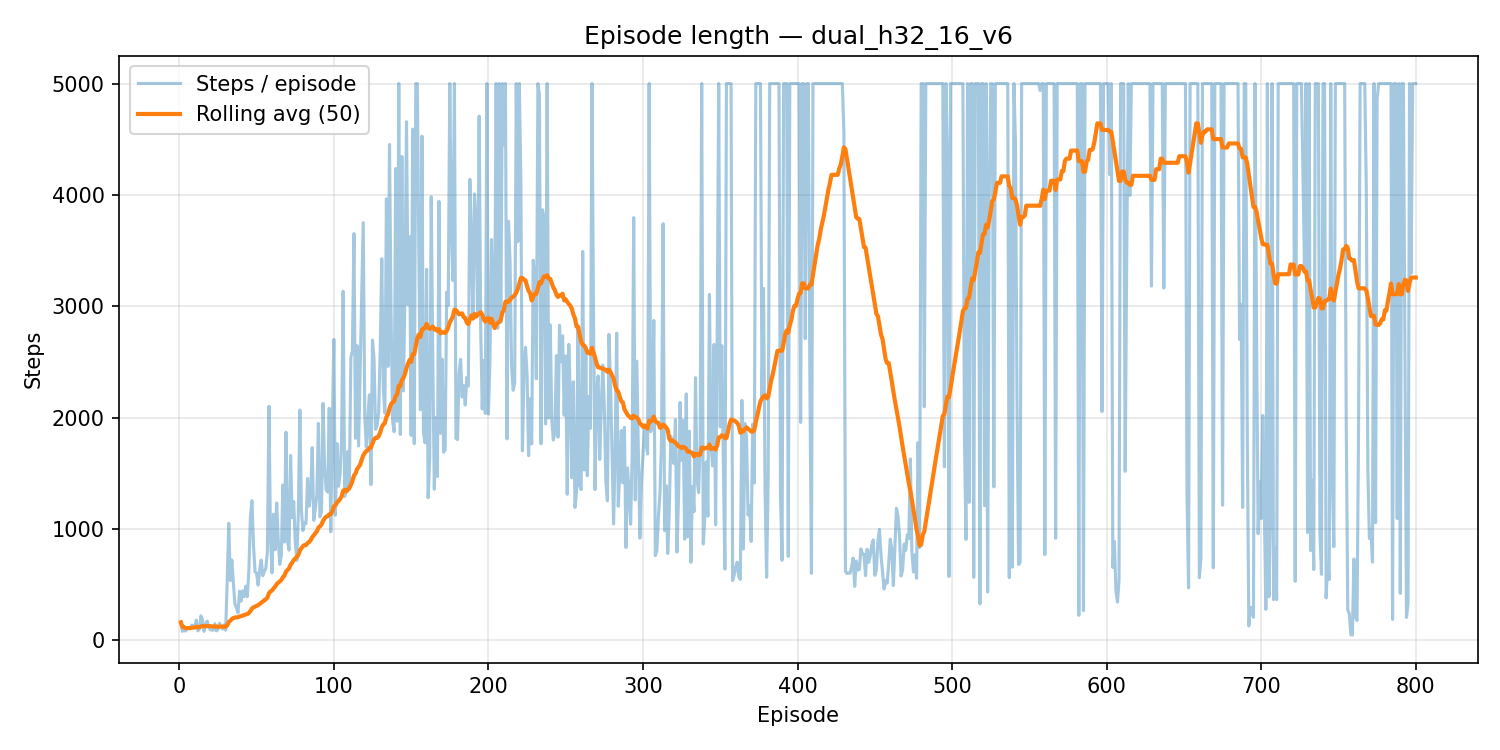
\includegraphics[width=0.48\linewidth]{artifacts/runs/dual_h32_16_v6/learning_curve_steps.png}%
 \hfill
 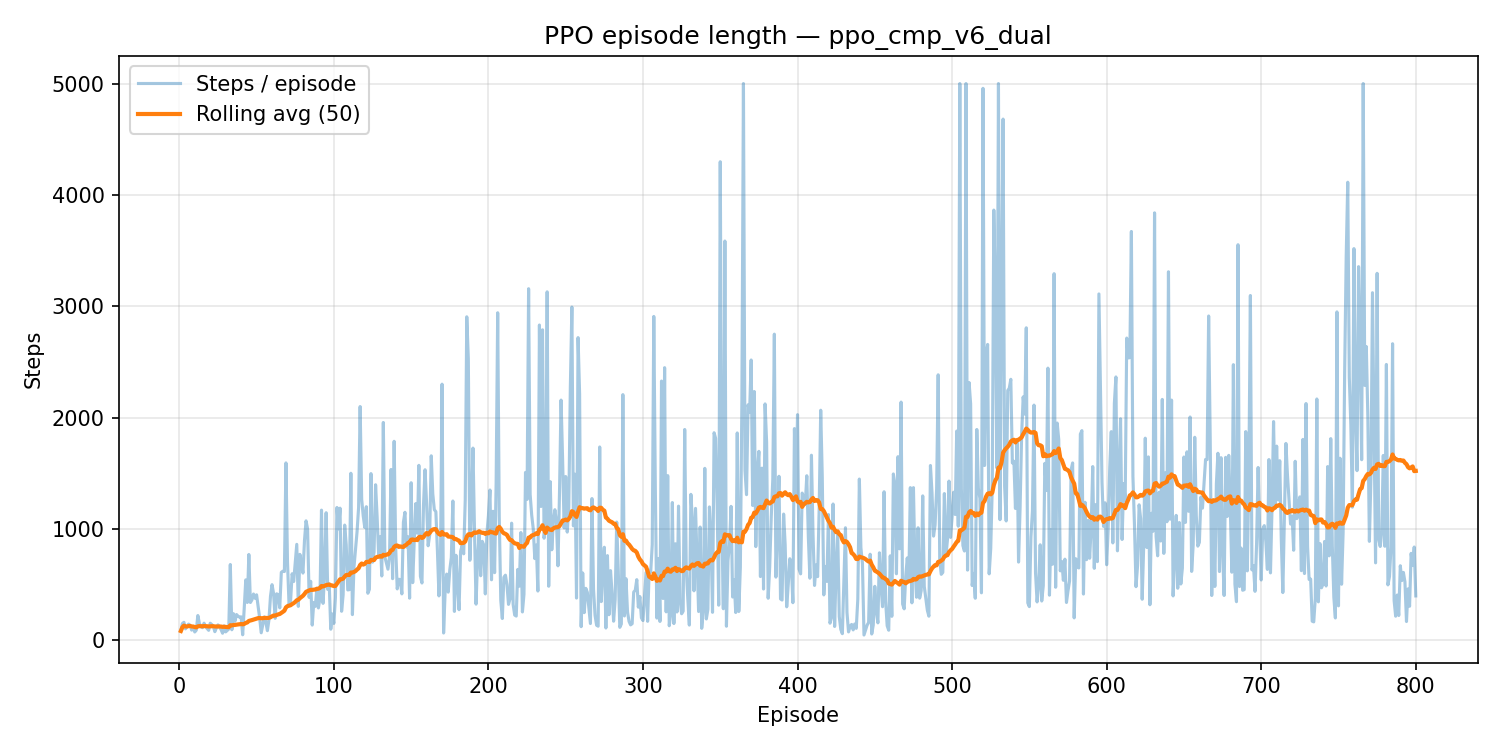
\includegraphics[width=0.48\linewidth]{artifacts/runs/ppo_cmp_v6_dual/learning_curve_steps.png}%
 \caption{Długość epizodu: SAC (\texttt{dual\_h32\_16\_v6}, lewy) i PPO (\texttt{ppo\_cmp\_v6\_dual}, prawy).}
 \label{Fig:cmp_steps}
\end{figure}

Ponieważ funkcja nagrody jest wspólna, można porównać także sumę nagrody w epizodzie (rys.~\ref{Fig:cmp_reward}). SAC generuje dodatnie nagrody epizodu po opanowaniu zadania; PPO pozostaje głównie w reżimie ujemnym (wczesne upadki i kary skalowane czasem).

\begin{figure}[H]
 \centering
 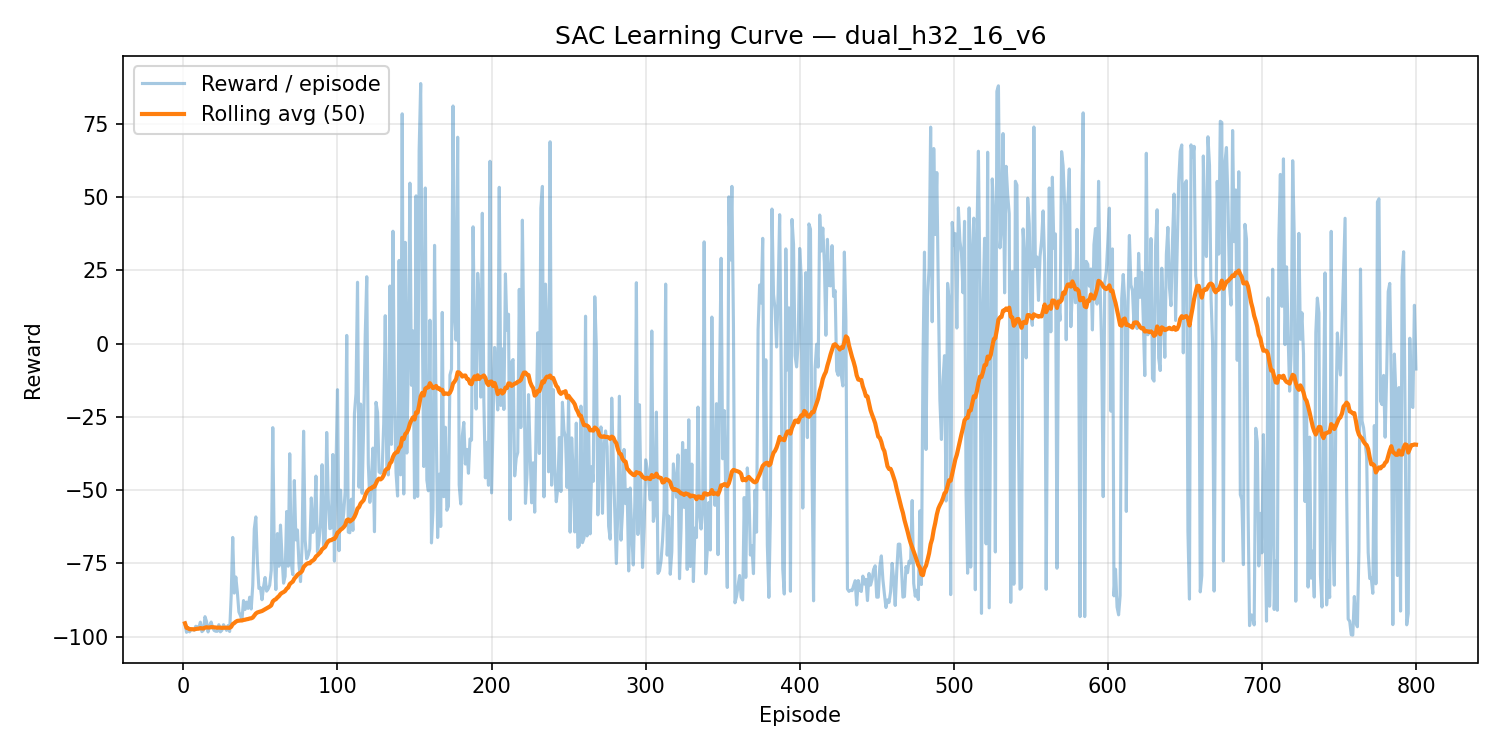
\includegraphics[width=0.48\linewidth]{artifacts/runs/dual_h32_16_v6/learning_curve.png}%
 \hfill
 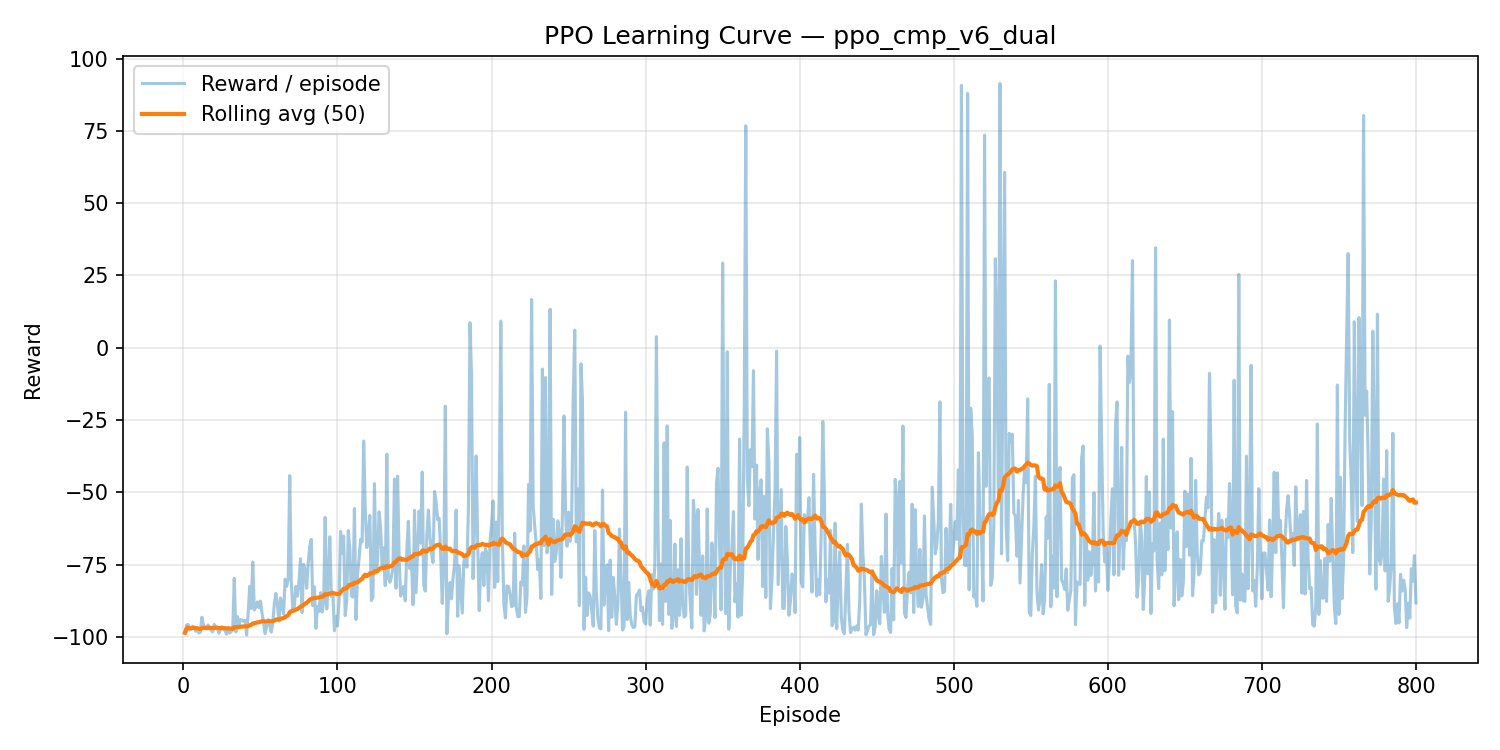
\includegraphics[width=0.48\linewidth]{artifacts/runs/ppo_cmp_v6_dual/learning_curve.png}%
 \caption{Nagroda epizodu: SAC (lewy) i PPO (prawy), ta sama funkcja celu.}
 \label{Fig:cmp_reward}
\end{figure}

\subsection{Różnice w hiperparametrach algorytmów}

Przy identycznym MDP algorytmy różnią się jedynie mechanizmem optymalizacji:

\begin{table}[H]
\centering
\renewcommand{\arraystretch}{1.2}
\begin{tabular}{|l|l|l|}
\hline
\textbf{Parametr} & \textbf{SAC} & \textbf{PPO} \\
\hline
Typ uczenia & off-policy & on-policy \\
Bufor / rollout & replay 50\,000, batch 128 & rollout 2048, 10 epok PPO \\
Entropia & $\alpha$: 0,35 $\rightarrow$ 0,15 & współczynnik entropii 0,01 \\
Learning rate & $3 \times 10^{-4} \rightarrow 10^{-4}$ & stałe $3 \times 10^{-4}$ \\
\hline
\end{tabular}
\caption{Główne różnice konfiguracji treningowej (środowisko identyczne)}
\label{tab:sac_ppo_hparams}
\end{table}

\subsection{Wnioski}

Przy identycznej fizyce, obserwacji \texttt{imu\_raw12}, akcji dwuwymiarowej i funkcji nagrody SAC osiąga wyraźnie lepsze wyniki niż PPO --- zarówno w treningu (Avg50 steps: 5000 wobec 1902), jak i w ewaluacji po zakończeniu uczenia (100\% wobec 6\% pełnych epizodów). PPO wykazuje zdolność do uczenia, co widać po rosnącym trendzie na wykresie długości epizodu, lecz w przeprowadzonym eksperymencie nie osiągnął stabilizacji na poziomie SAC w ciągu 800 epizodów. Dalszy postęp PPO wymagałby prawdopodobnie dłuższego treningu lub strojenia hiperparametrów, takich jak $\varepsilon$, \texttt{rollout\_steps} czy harmonogram współczynnika uczenia.

Główną przyczynę przewagi SAC należy przypisać uczeniu \emph{off-policy}: algorytm efektywniej wykorzystuje próbki zgromadzone w buforze doświadczeń, a eksploracja sterowana entropią ułatwia odkrycie stabilnej polityki przy długim horyzoncie ($\gamma = 0{,}999$ i 5000 kroków na epizod). Ze względu na wyniki porównawcze do wdrożenia na Raspberry Pi wybrano politykę SAC z runu \texttt{dual\_h32\_16\_v6}. PPO pełni natomiast rolę drugiego, wymaganego algorytmu RL --- z pełną implementacją w modułach \texttt{rl/ppo.py} i \texttt{train\_sim\_ppo.py} oraz przeprowadzonym eksperymentem porównawczym w tym samym środowisku symulacyjnym.

\clearpage

\addcontentsline{toc}{section}{Literatura}

\begin{thebibliography}{4}


\bibitem{str1}
http://jtjt.pl/odwrocone-wahadlo. Dostęp: 28.04.2026r.

\bibitem{str2}
https://scaron.info/robotics/wheeled-inverted-pendulum-model.html. Dostęp: 28.04.2026r.

\bibitem{str3}
https://pl.eitca.org/sztuczna-inteligencja/. Dostęp: 29.04.2026r.

\bibitem{str4}
https://www.flowhunt.io/pl/slownik/q-learning/. Dostęp: 29.04.2026r.

\bibitem{str5}
https://www.geeksforgeeks.org/machine-learning/q-learning-in-python/. Dostęp: 29.04.2026r.

\bibitem{str6}
Mishura, Y., Ralchenko, K. (2026). Differential Shannon and Rényi entropies revisited. Lithuanian Mathematical Journal.

\bibitem{str7}
Nalewajski, R.F. (2011). Elements of Information Theory. In: Perspectives in Electronic Structure Theory. Springer, Berlin, Heidelberg.

\bibitem{str8}
Rudin W. (1953r.). Principles of Mathematical Analysis.

\bibitem{str9}
Jonathan H. Connell and Sridhar Mahadevan, Kluwer, Boston, 1993/1997. Robot Learning.

\bibitem{str10}
Haarnoja, T., Zhou, A., Abbeel, P. Levine, S.. (2018). Soft Actor-Critic: Off-Policy Maximum Entropy Deep Reinforcement Learning with a Stochastic Actor. 

\bibitem{str11}
Schulman, J., Wolski, F., Dhariwal, P., Radford, A., & Klimov, O. (2017). Proximal Policy Optimization Algorithms.

\bibitem{str12}
Schulman, J., Levine, S., Abbeel, P., Jordan, M., & Moritz, P. (2015). Trust Region Policy Optimization.

\bibitem{str13}
Schulman, J., Moritz, P., Levine, S., Jordan, M., & Abbeel, P. (2015). High-Dimensional Continuous Control Using Generalized Advantage Estimation.

\bibitem{str14}
Sutton, R. S., & Barto, A. G. (2018). Reinforcement Learning: An Introduction. MIT Press.









% \bibitem{str6}
% https://semcore.pl/czym-jest-i-jak-dziala-narzedzie-pytorch/. Dostęp: 30.04.2026r.

% \bibitem{str7}
% https://docs.pytorch.org/docs/2.11/index.html. Dostęp: 30.04.2026r.





% \bibitem{str} http://weii.portal.prz.edu.pl/pl/materialy-do-pobrania. Dostęp 5.01.2015.
% \bibitem{Jakubczyk1997} Jakubczyk T., Klette A.: Pomiary w akustyce. WNT, Warszawa 1997.
% \bibitem{Barski2011} Barski S.: Modele transmitancji. Elektronika praktyczna, nr 7/2011, str. 15-18.
% \bibitem{dokum} Czujnik S200. Dokumentacja techniczno-ruchowa. Lumel, Zielona Góra, 2001.
% \bibitem{Pawluk2001} Pawluk K.: Jak pisać teksty techniczne poprawnie, Wiadomości Elektrotechniczne, Nr 12, 2001, str. 513-515.
\end{thebibliography}

\end{document} 
